\documentclass{article}

\usepackage[ngerman]{babel}
\usepackage[T1]{fontenc}
\usepackage[utf8]{inputenc}
\usepackage{float}
\usepackage{svg}
\usepackage{amsmath}
\usepackage{parskip}
\usepackage{csquotes}
\usepackage[hidelinks]{hyperref}
\usepackage{float}
\usepackage{listings}
\usepackage{xcolor}
\usepackage{todonotes}
\usepackage{geometry}

\geometry{
    a4paper,
    total={140mm,237mm},
    left=35mm,
    top=40mm,
}

\lstdefinestyle{matlab}{
    language=Matlab,
    basicstyle=\ttfamily\small,
    commentstyle=\color{green!50!black},
    keywordstyle=\color{blue},
    numbers=none,
    frame=none,
    breaklines=true,
    breakatwhitespace=true,
    tabsize=4,
    xleftmargin=15pt
}




\pagestyle{empty}

\title{
    \textbf{Database I} \\
    \textbf{IoT Solutions Inc. } \\
    \vspace{2em}
    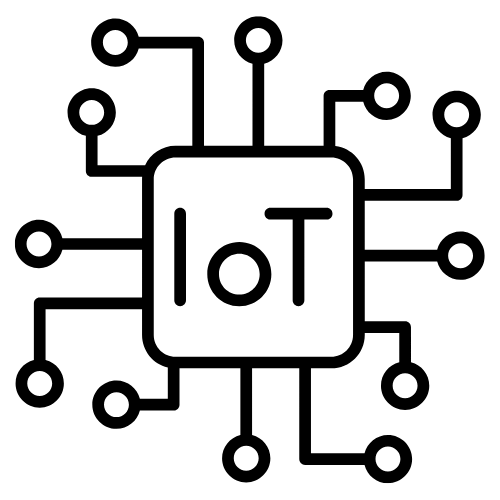
\includegraphics[width=0.5\linewidth]{img/title.png} 
}

\author{
    \vspace{8em} \\
    \textbf{Matrikelnr.:} \\
    \textbf{Dozent:} apl. Prof. Dr. Nuo Li \\
    \textbf{Kurs:} Database\\
    \textbf{Application:}  DB Design \\
    \vspace{8em} 
}
\date{\today}



\begin{document}


\maketitle

% \include{vorgehen_regelungstechnik}



\newpage
\section{Intruduction}

We as \textbf{IoT Solutions Inc. } are a company specializing in the management of IoT (Internet of Things) devices across various sectors. We provide innovative solutions for industries such as healthcare, industrial operations, and smart home automation, whereas smart home devices are provided to endusers or small businesses. 
Our Productline consists of a wide range of IoT devices, including security cameras, health monitors and also industrial sensors. 

\subsection{ER/EER Model}
The ER/EER Model is designed to provide a comprehensive overview of the relationships between different entities in our system. The model includes the following entities: 

\begin{figure}[H]
\centering
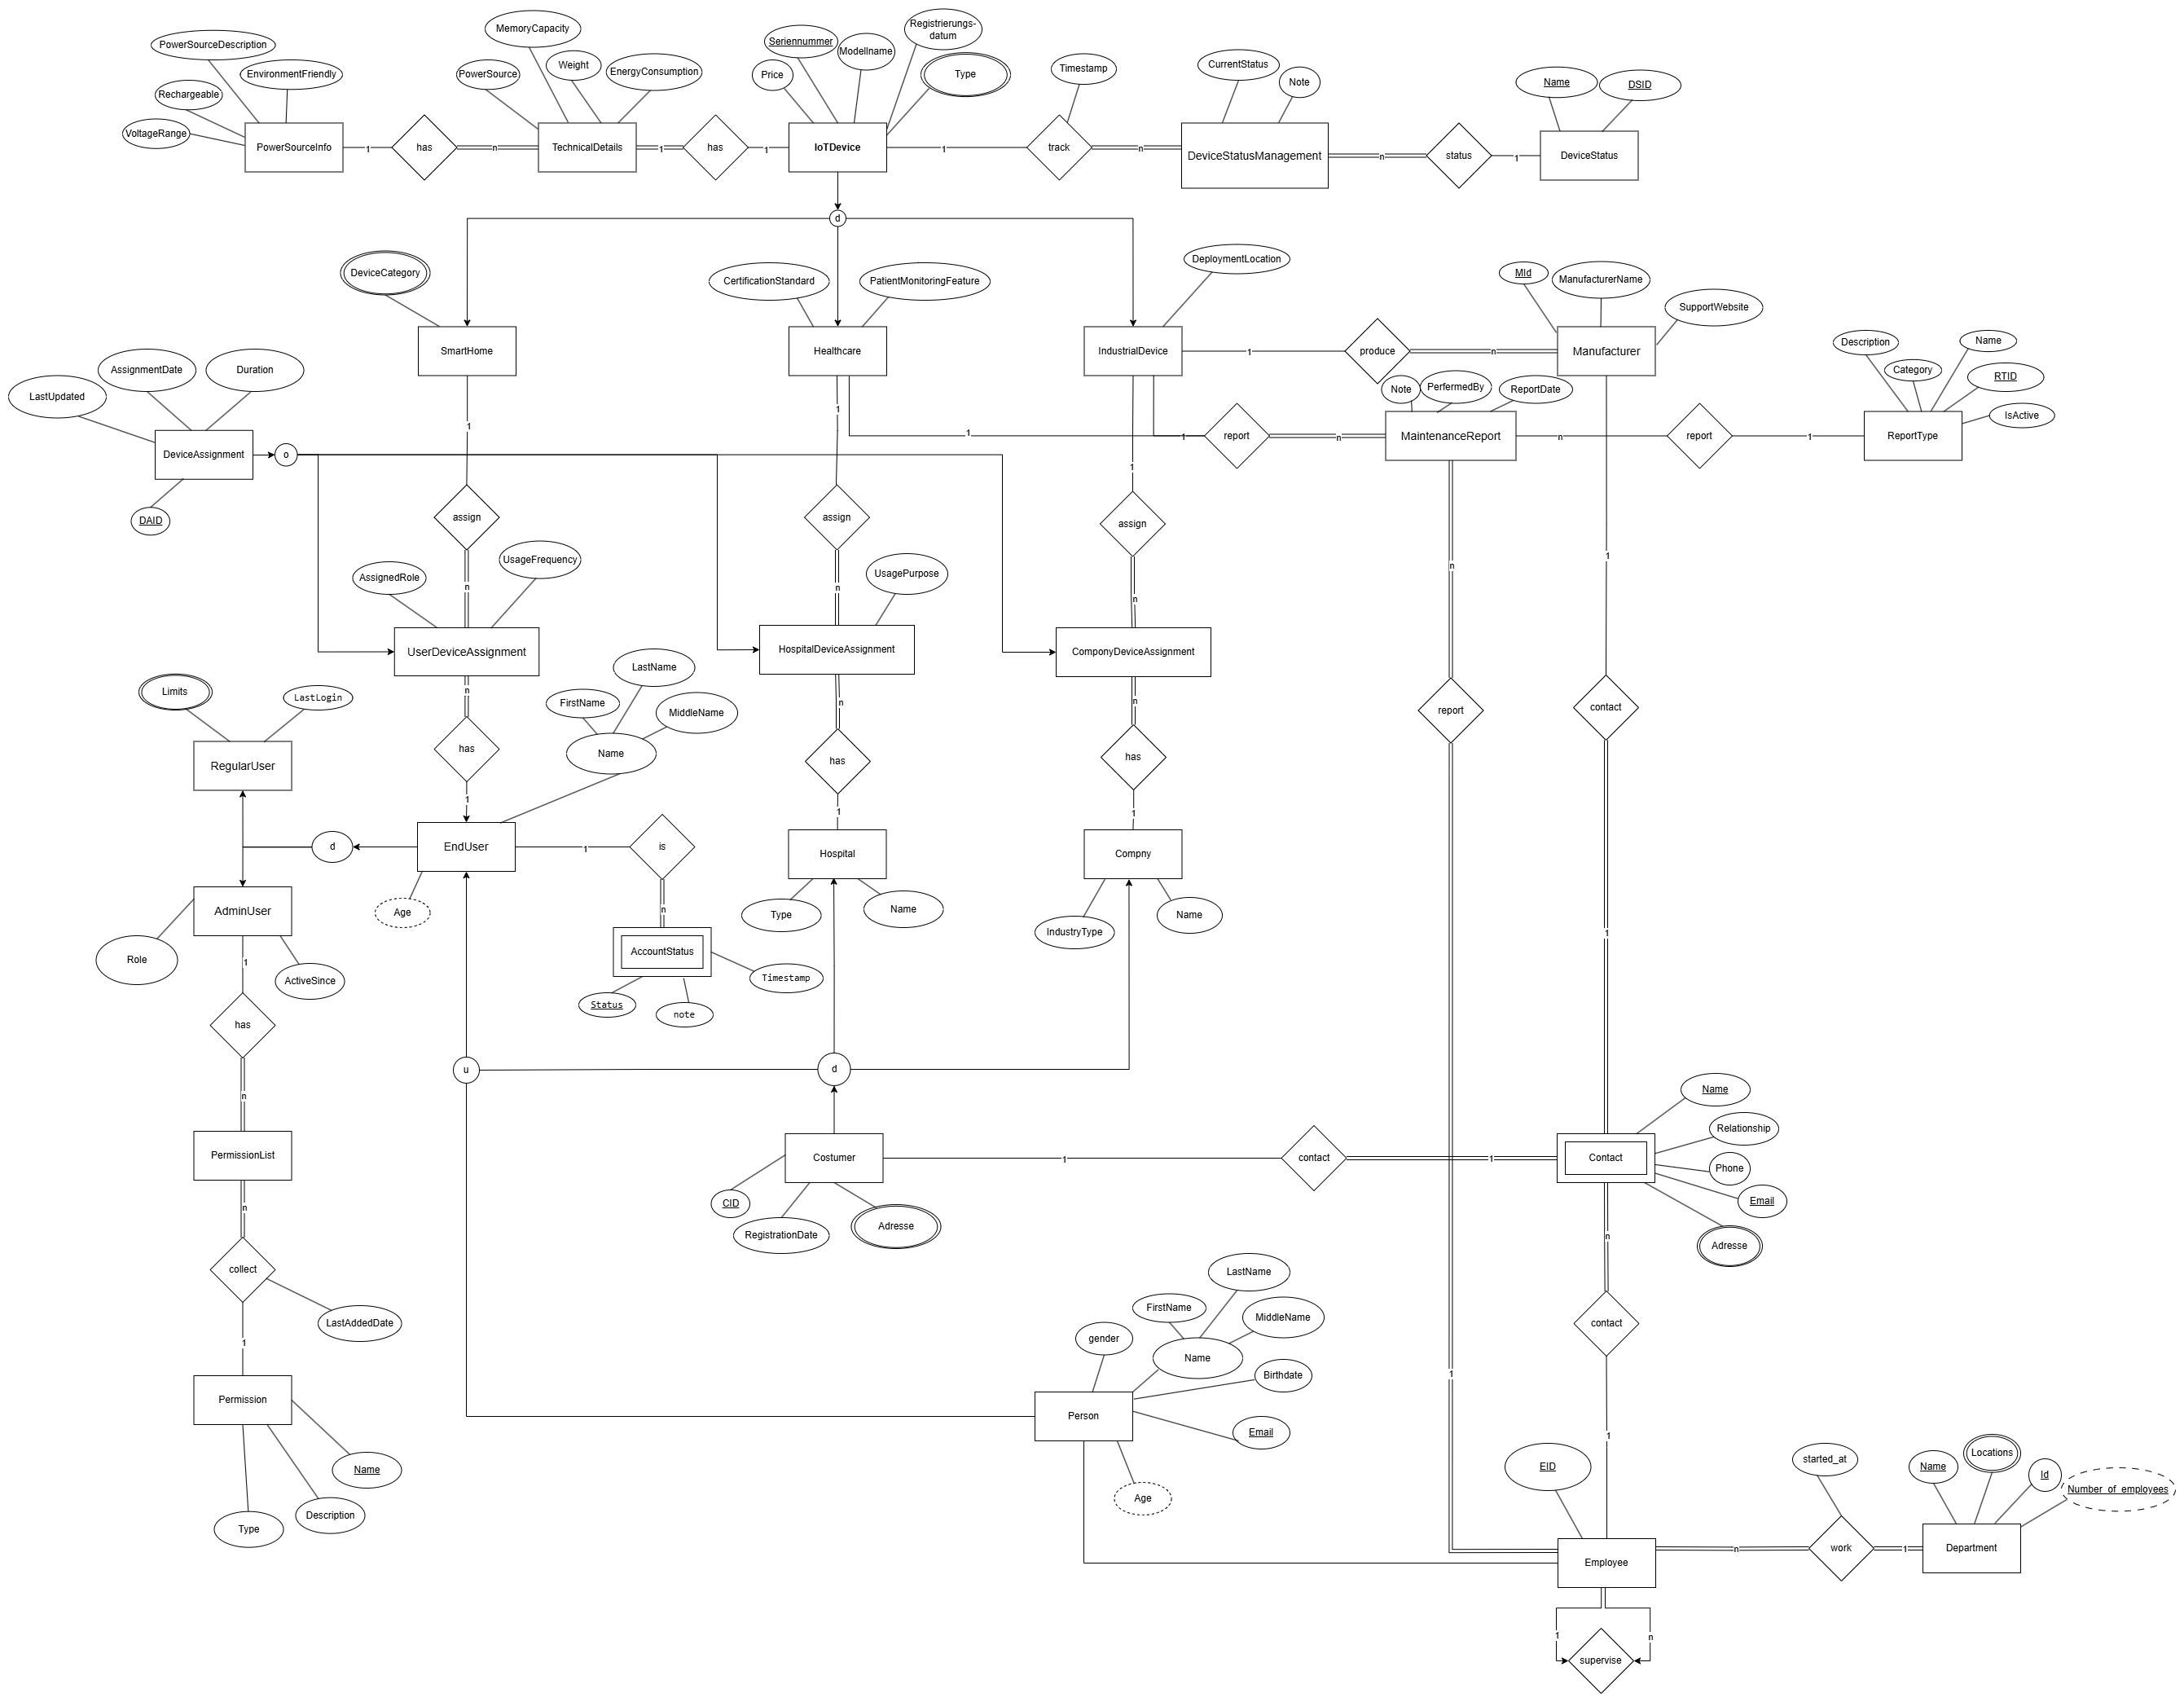
\includegraphics[width=\linewidth]{img/EER.png}
\end{figure}




\textbf{ IoTDevice :}
This entity is the foundation of the system, representing the physical IoT devices being managed. Each device needs unique identifiers, such as serial numbers and model names, as well as attributes to track its registration and operational state.




\begin{itemize}
    \item \textbf{IndustrialDevice (Inherited from IoTDevice):}
    This entity represents IoT devices used in industrial settings. 
    \item \textbf{SmartHomeDevice (Inherited from IoTDevice):}
    This entity is Specialization for IoT devices used in smart home environments.
    \item \textbf{HealthcareIoTDevice (Inherited from IoTDevice):} This entity is specialized for healthcare-related IoT devices.
\end{itemize}


\textbf{Customer:}
Represents the companies or individuals who purchase or use IoT devices managed by the system. Customers are often linked to specific device assignments.

\begin{itemize}
    \item \textbf{Enduser (Inherited from Customer):} customers who are private individuals using IoT devices for personal purposes, such as smart home devices.
        \begin{itemize}
            \item \textbf{RegularUser} Represents typical users with standard permissions and limited access to device configurations.
            \item \textbf{AdminUser:} Represents users with elevated privileges for managing the their own devices, or other users.
        \end{itemize}

    \item \textbf{Hospital (Inherited from Customer):} Represents organizations or Hospitals purchasing or managing IoT devices.
    \item \textbf{Compny (Inherited from Customer):} Represents organizations or companies purchasing or managing IoT devices for business purposes.
\end{itemize}

\textbf{DeviceAssignment:}
This Entity tracks the assignment of devices to entities like users, hospitals, or companies.
\begin{itemize}
    \item \textbf{HospitalDeviceAssignment:} Represents devices assigned to hospitals for healthcare-specific use cases.
    \item \textbf{CompanyDeviceAssignment:} Represents devices assigned to companies for business or industrial use.
    \item \textbf{UserDeviceAssignment:} Represents devices assigned to individual users (e.g., for personal or smart home use).
\end{itemize}

\textbf{Manufacturer:}
Represents the companies that produce part of IoT devices, specifically industrial devices. The \textbf{IoT Solutions Inc. } then assemble it together and sell it as its own product. 


\newpage
\section{Normalization}
\textbf{1NF:} The data is organized into tables, and each table has a primary key. Each attribute in the table contains atomic values, and there are no repeating groups or arrays. As an example, \textbf{Person} table has a composed value for the attribute \textbf{name} which consists of \textbf{first name}, \textbf{last name} and \textbf{middle name}. This is not atomic and should be separated into three different attributes.
\begin{figure}[H]
\centering
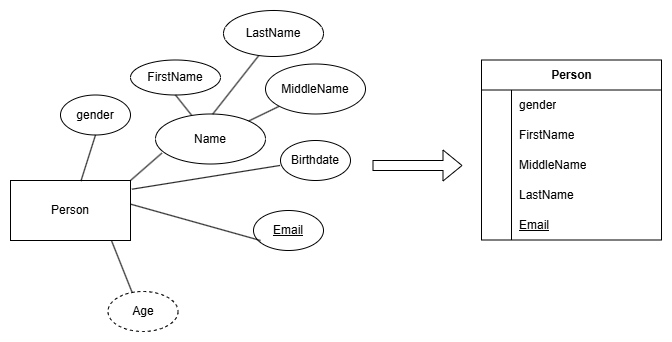
\includegraphics[width=\linewidth]{img/1nf.png}
\caption{1NF Normalization based on the Person table.}
\end{figure}

\textbf{2NF:} All non-key attributes are fully functionally dependent on the primary key. as an example the \textbf{TechnicalDetails} table has two primary keys, \textbf{TDID} and \textbf{PowerSource}. All non-key attributes are not fully functionally dependent on the primary key, as for example powerSourceDescription, environmentfriendly or rechargeable attributes depends on the attribute PowerSource. This means that for selecting the powerSourceDescription, environmentfriendly or rechargeable attributes, we need to combine the two primary keys. This is not 2NF, so we could decompose the table into two tables, one for the power source and one for the technical details. The power source table will have the primary key PowerSource and the technical details table will have the primary key TDID. The power source table will have the attributes PowerSourceDescription, environmentfriendly and rechargeable. The technical details table will have all remaining attributes. This way, we can select the power source description, environment friendly or rechargeable attributes without having to combine the two primary keys.
\begin{figure}[H]
\centering
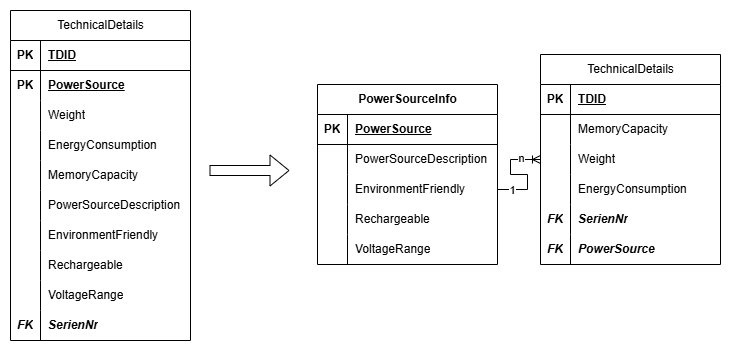
\includegraphics[width=\linewidth]{img/2nf.png}
\caption{2NF Normalization based on the TechnicalDetails table.}
\end{figure}



\textbf{3NF:} All transitive dependencies are removed. This means that all non-key attributes are not dependent on other non-key attributes. As an example, the \textbf{Adress} table has a transitive dependency on the \textbf{city}, \textbf{postcode} and \textbf{country} attributes. This means that city is dependent on the postcode attribute and the postcode is dependent on the country attribute. This is not 3NF, so we could decompose the table into three tables, one for the postcodeInfo, one for the Address. 
\begin{figure}[H]
\centering
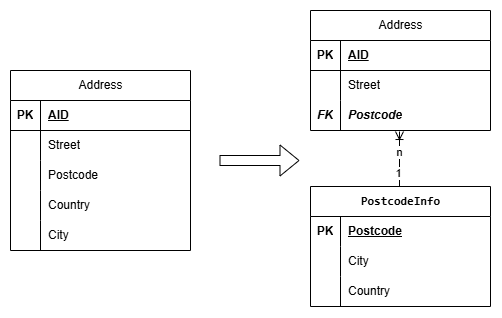
\includegraphics[width=\linewidth]{img/3nf.png}
\caption{3NF Normalization based on the Address table.}
\end{figure}


\newpage
\section{Implementation screenshots}


\subsection{Creating tables}
\begin{figure}[H]
\centering
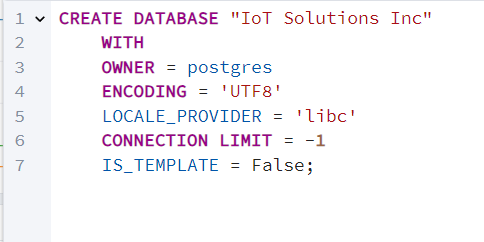
\includegraphics[width=\linewidth]{img/iot_solution_inc_db.png}
\caption{Iot Solution Inc Databse}
\end{figure}

\begin{figure}[H]
\centering
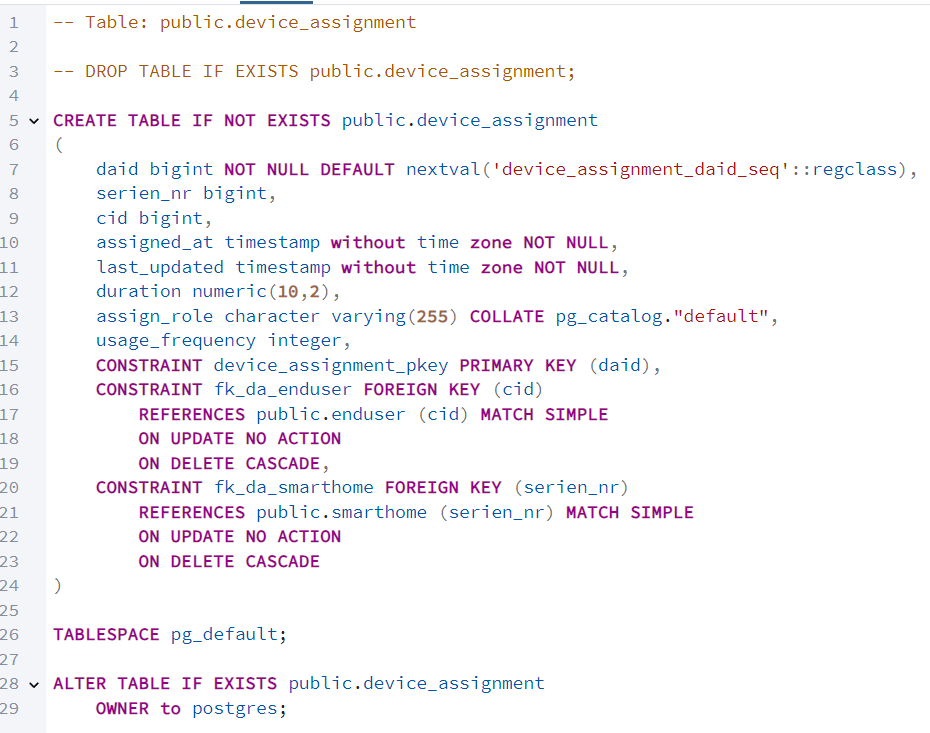
\includegraphics[width=\linewidth]{img/device_assignment.png}
\caption{device assignment table}
\end{figure}


\begin{figure}[H]
\centering
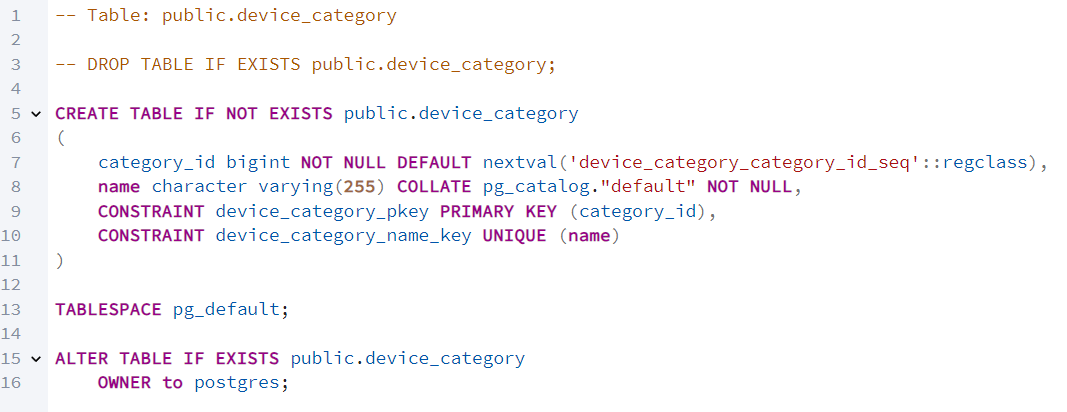
\includegraphics[width=\linewidth]{img/device_category.png}
\caption{device category table}
\end{figure}


\begin{figure}[H]
\centering
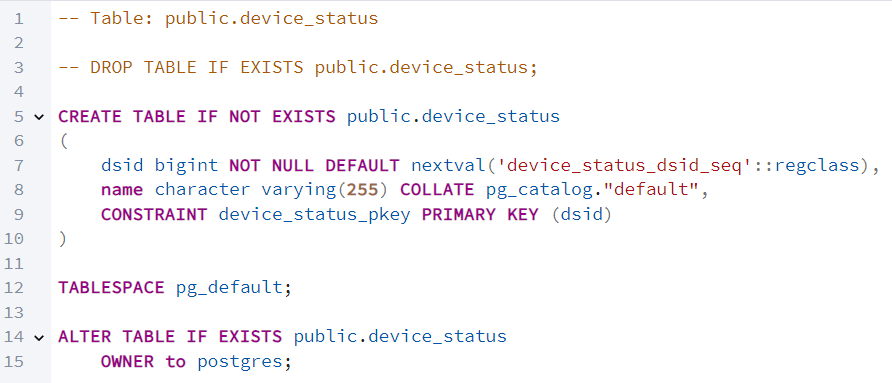
\includegraphics[width=\linewidth]{img/device_status.png}
\caption{device status table}
\end{figure}

\begin{figure}[H]
\centering
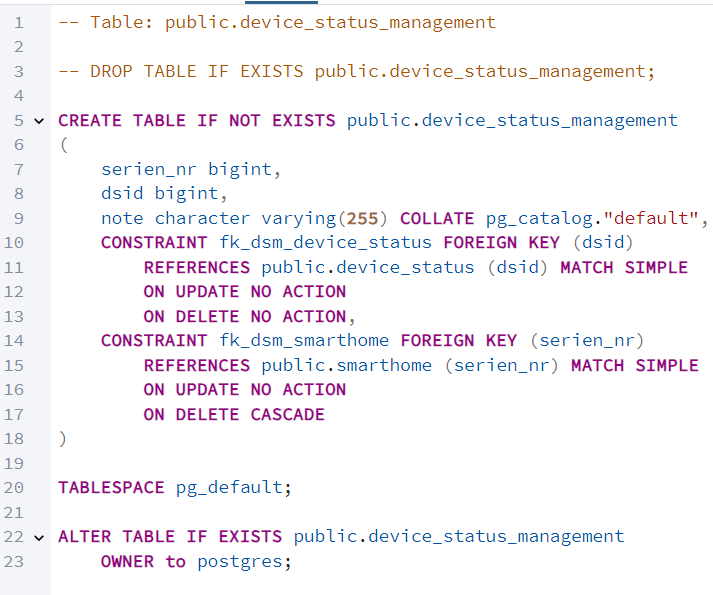
\includegraphics[width=\linewidth]{img/device_status_managment.png}
\caption{device status managment table}
\end{figure}


\begin{figure}[H]
\centering
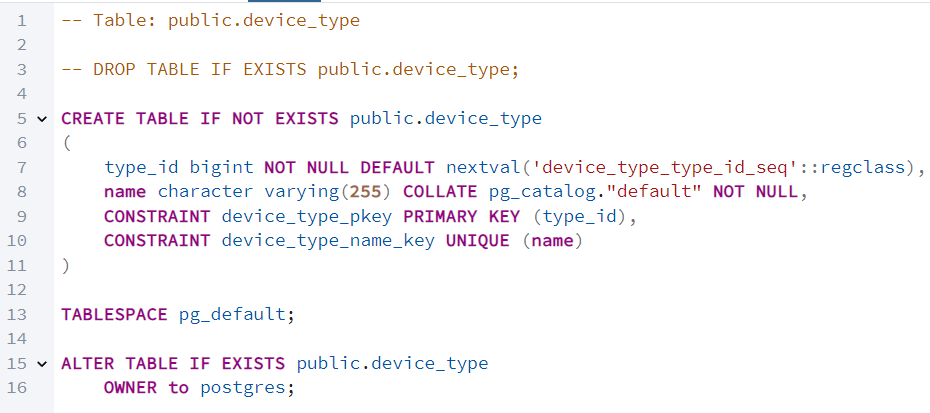
\includegraphics[width=\linewidth]{img/device_type.png}
\caption{device type table}
\end{figure}

\begin{figure}[H]
\centering
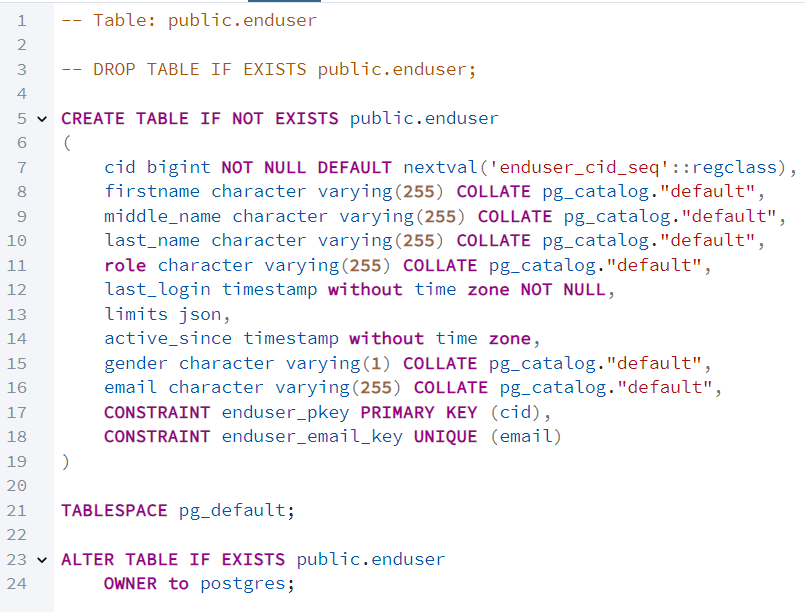
\includegraphics[width=\linewidth]{img/enduser.png}
\caption{enduser table}
\end{figure}


\begin{figure}[H]
\centering
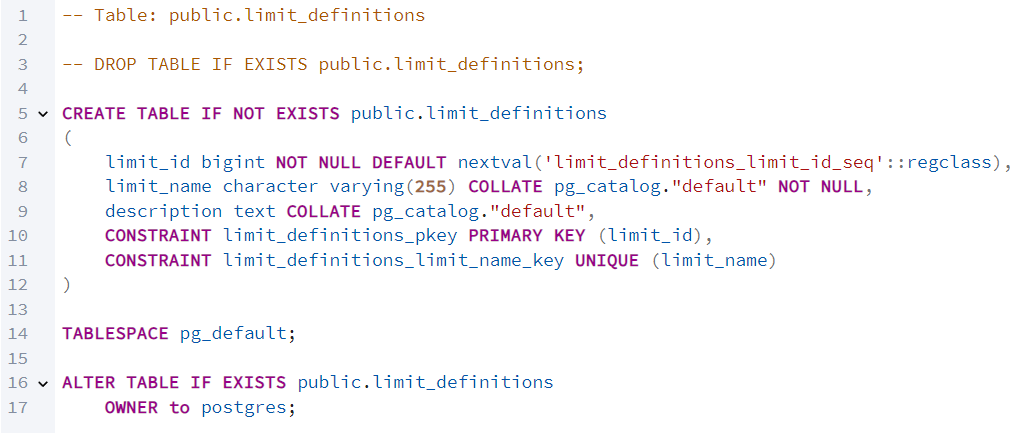
\includegraphics[width=\linewidth]{img/limit_definitions.png}
\caption{limit definition table}
\end{figure}


\begin{figure}[H]
\centering
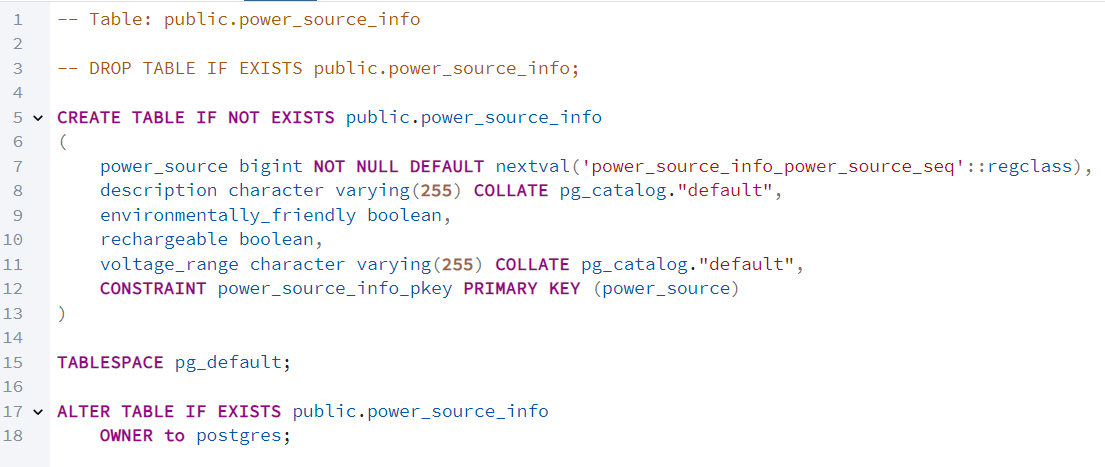
\includegraphics[width=\linewidth]{img/power_source_info.png}
\caption{power source Info table}
\end{figure}

\begin{figure}[H]
\centering
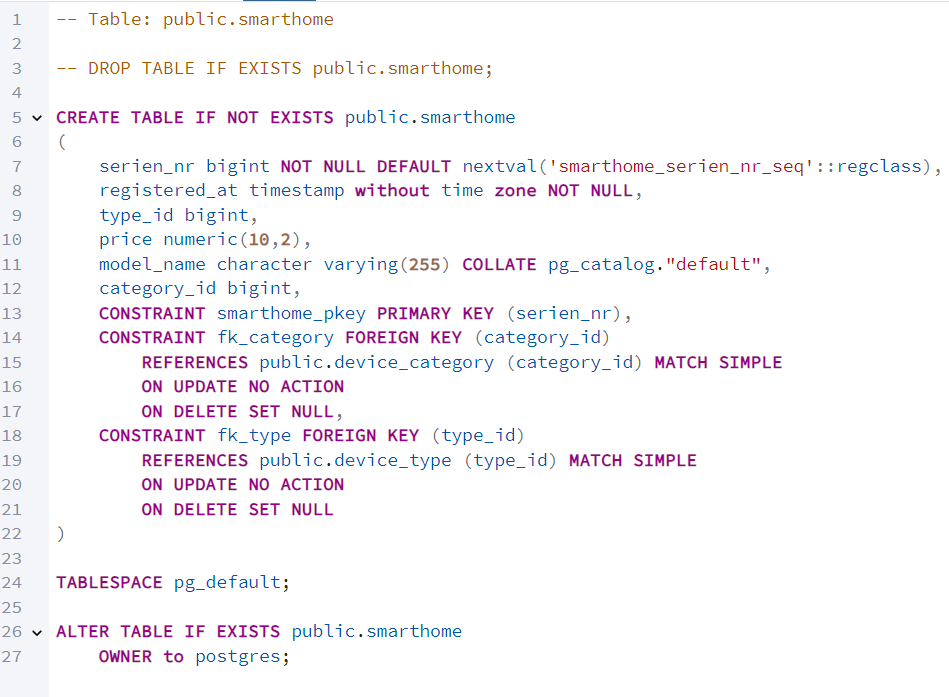
\includegraphics[width=\linewidth]{img/smarthome.png}
\caption{smarthome table}
\end{figure}


\begin{figure}[H]
\centering
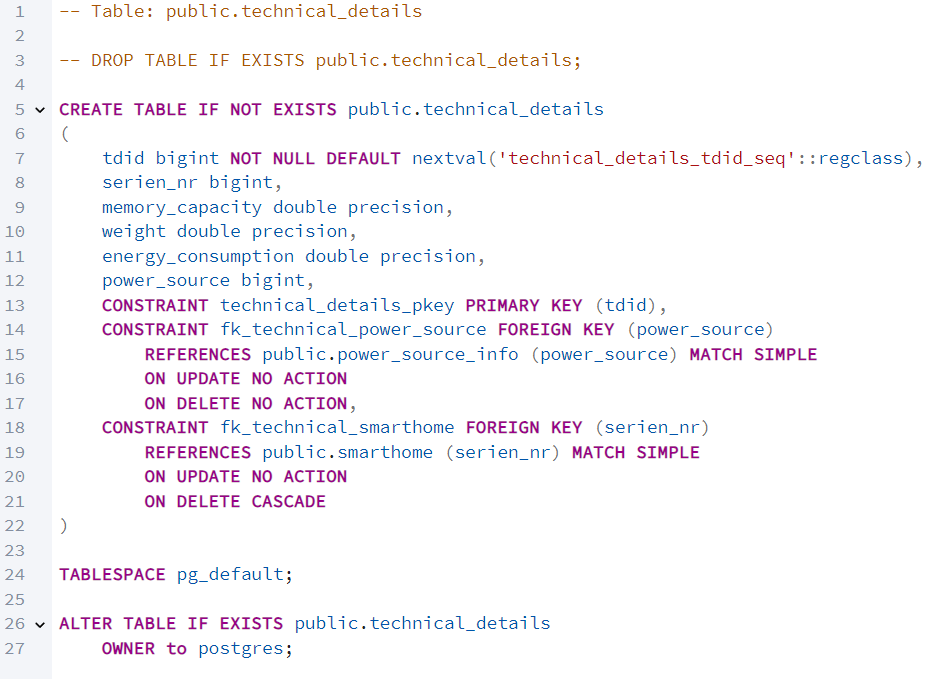
\includegraphics[width=\linewidth]{img/technical_details.png}
\caption{technical details table}
\end{figure}

\begin{figure}[H]
\centering
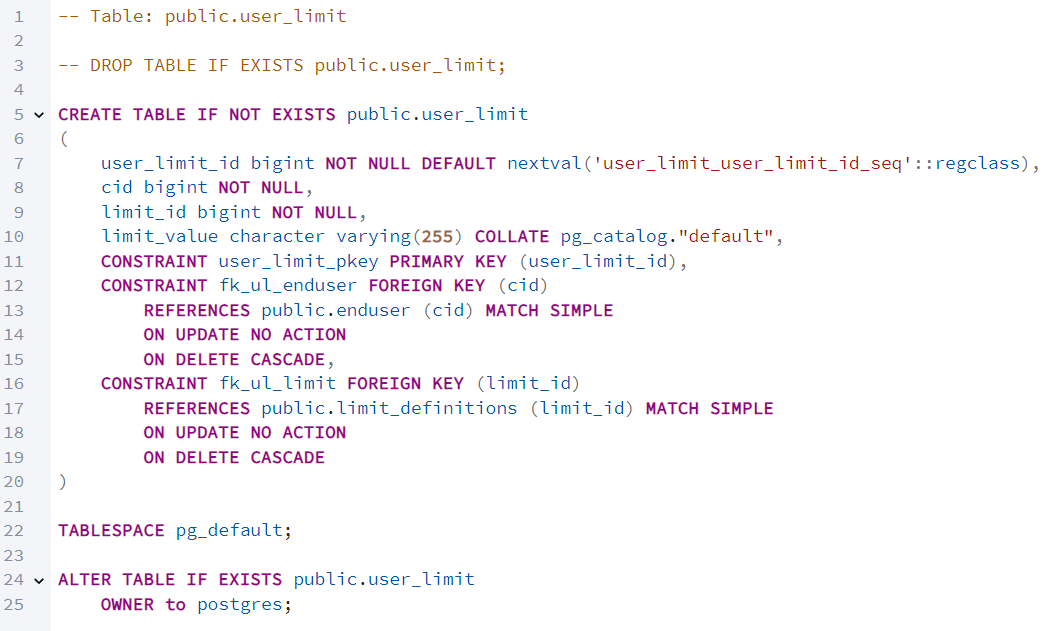
\includegraphics[width=\linewidth]{img/user_limit.png}
\caption{user limit table}
\end{figure}


\subsection{Queries}

\begin{figure}[H]
\centering
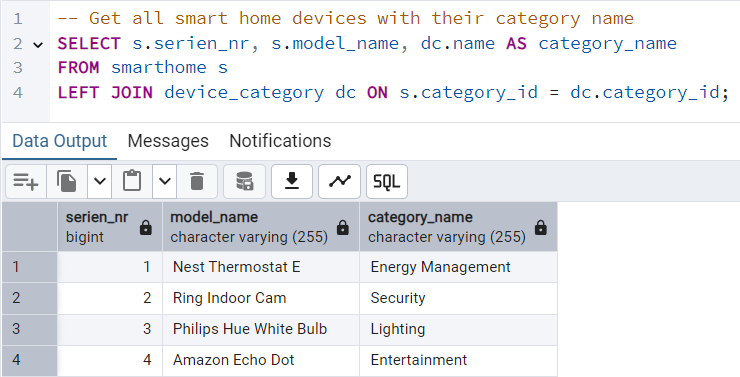
\includegraphics[width=\linewidth]{img/q1.png}
\caption{Get all smart home devices with their category name}
\end{figure}


\begin{figure}[H]
\centering
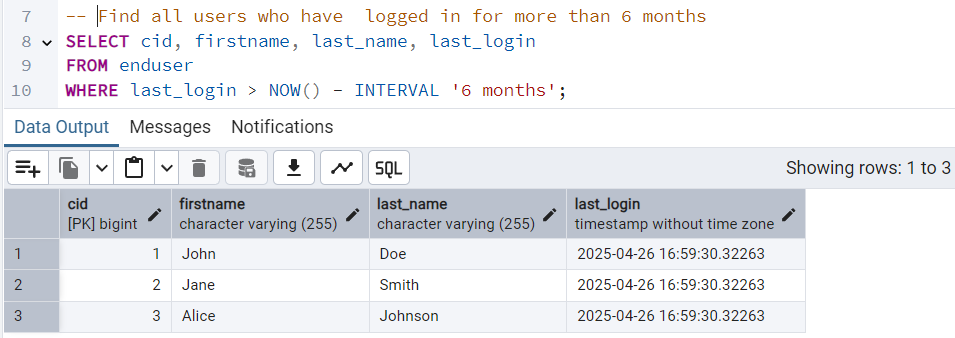
\includegraphics[width=\linewidth]{img/q2.png}
\caption{Find all users who have logged in for more than 6 months}
\end{figure}


\begin{figure}[H]
\centering
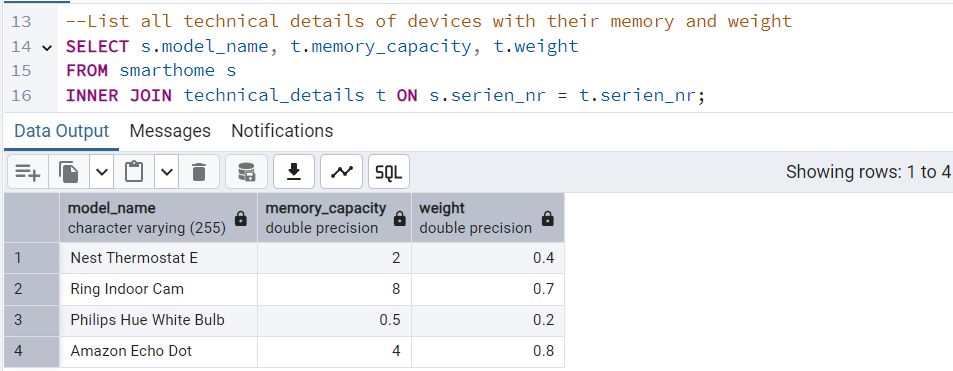
\includegraphics[width=\linewidth]{img/q3.png}
\caption{List all technical details of devices with their memory and weight}
\end{figure}

\begin{figure}[H]
\centering
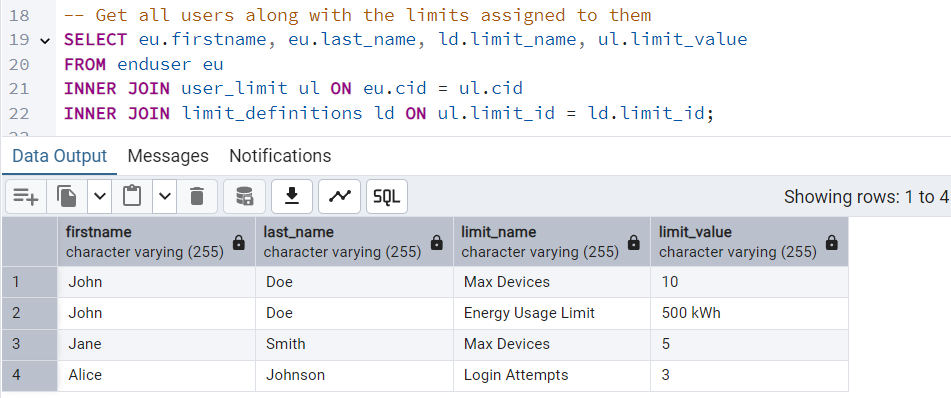
\includegraphics[width=\linewidth]{img/q4.png}
\caption{Get all users along with the limits assigned to them}
\end{figure}

\begin{figure}[H]
\centering
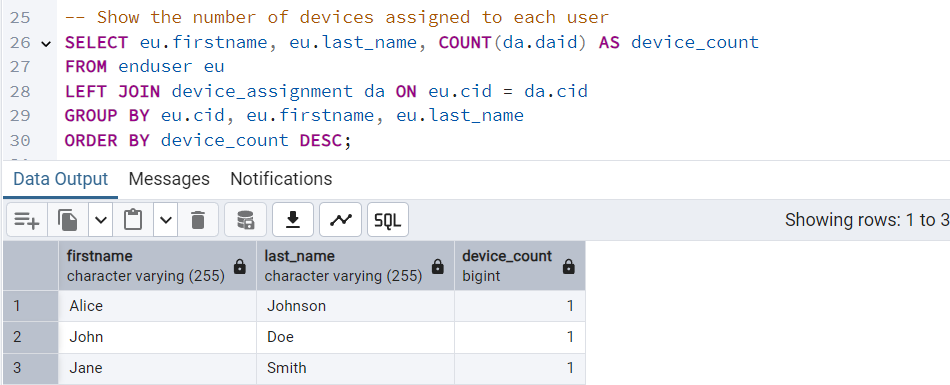
\includegraphics[width=\linewidth]{img/q5.png}
\caption{Show the number of devices assigned to each user}
\end{figure}


\begin{figure}[H]
\centering
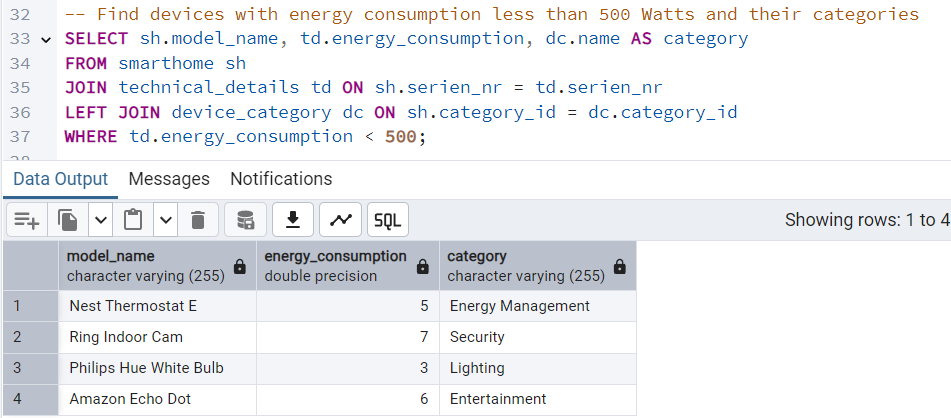
\includegraphics[width=\linewidth]{img/q6.png}
\caption{Find devices with energy consumption less than 500 Watts and their categories}
\end{figure}



\end{document}